

\documentclass[border=10pt]{standalone}

\usepackage{amsmath}
\usepackage{amssymb}
\usepackage{tikz}
\usetikzlibrary{positioning, arrows.meta, fit, calc}

\begin{document}
	
	% ============================================================
	% VAE Computation Graph
	% ============================================================
	
	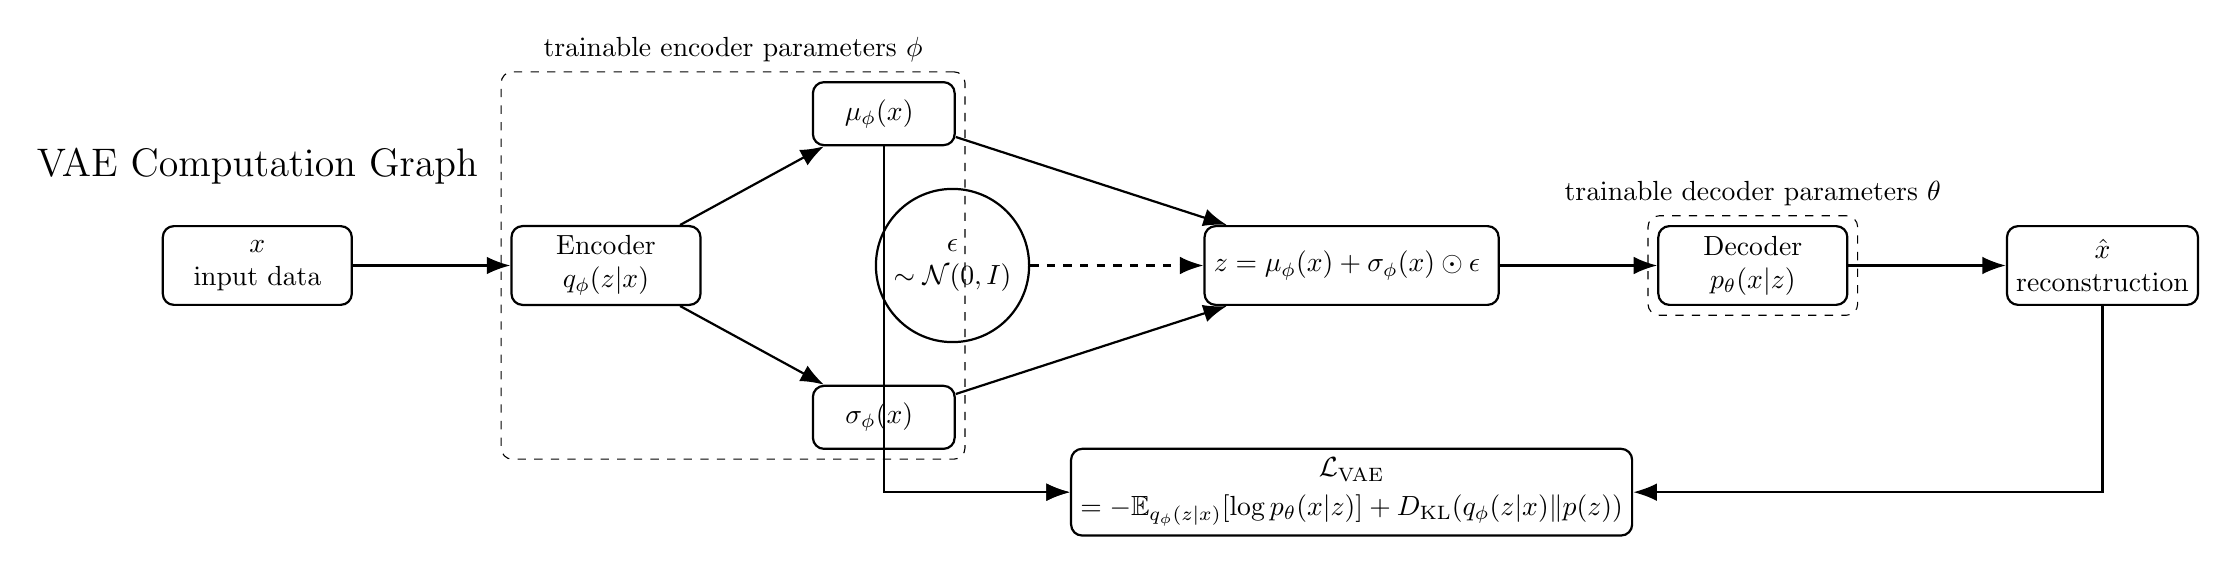
\begin{tikzpicture}[
		node distance=1.6cm and 2.0cm,
		box/.style={
			rectangle,
			rounded corners,
			draw,
			thick,
			align=center,
			minimum width=2.4cm,
			minimum height=1.0cm
		},
		smallbox/.style={
			rectangle,
			rounded corners,
			draw,
			thick,
			align=center,
			minimum width=1.8cm,
			minimum height=0.8cm
		},
		stochastic/.style={
			circle,
			draw,
			thick,
			align=center,
			minimum size=1.1cm
		},
		arrow/.style={
			-{Latex[length=3mm]},
			thick
		},
		dashedarrow/.style={
			-{Latex[length=3mm]},
			thick,
			dashed
		}
		]
		
		\node[box] (x) {$x$\\input data};
		
		\node[box, right=of x] (enc) {
			Encoder\\
			$q_\phi(z|x)$
		};
		
		\node[smallbox, above right=1.0cm and 1.4cm of enc] (mu) {
			$\mu_\phi(x)$
		};
		
		\node[smallbox, below right=1.0cm and 1.4cm of enc] (sigma) {
			$\sigma_\phi(x)$
		};
		
		\node[stochastic, right=2.2cm of enc] (eps) {
			$\epsilon$\\
			$\sim \mathcal{N}(0,I)$
		};
		
		\node[box, right=2.2cm of eps] (z) {
			$z=\mu_\phi(x)+\sigma_\phi(x)\odot \epsilon$
		};
		
		\node[box, right=of z] (dec) {
			Decoder\\
			$p_\theta(x|z)$
		};
		
		\node[box, right=of dec] (xhat) {
			$\hat{x}$\\
			reconstruction
		};
		
		\node[box, below=1.8cm of z] (loss) {
			$\mathcal{L}_{\mathrm{VAE}}$\\[2pt]
			$=
			-\mathbb{E}_{q_\phi(z|x)}
			[\log p_\theta(x|z)]
			+
			D_{\mathrm{KL}}
			(q_\phi(z|x)\Vert p(z))$
		};
		
		\draw[arrow] (x) -- (enc);
		\draw[arrow] (enc) -- (mu);
		\draw[arrow] (enc) -- (sigma);
		\draw[arrow] (mu) -- (z);
		\draw[arrow] (sigma) -- (z);
		\draw[dashedarrow] (eps) -- (z);
		\draw[arrow] (z) -- (dec);
		\draw[arrow] (dec) -- (xhat);
		\draw[arrow] (xhat) |- (loss);
		\draw[arrow] (mu) |- (loss);
		\draw[arrow] (sigma) |- (loss);
		
		\node[
		draw,
		dashed,
		rounded corners,
		fit=(enc)(mu)(sigma),
		label=above:{trainable encoder parameters $\phi$}
		] {};
		
		\node[
		draw,
		dashed,
		rounded corners,
		fit=(dec),
		label=above:{trainable decoder parameters $\theta$}
		] {};
		
		\node[above=0.4cm of x] {\Large VAE Computation Graph};
		
	\end{tikzpicture}
	
	
	\vspace{1.5cm}
	
	
	% ============================================================
	% VeRA Computation Graph
	% ============================================================
	
	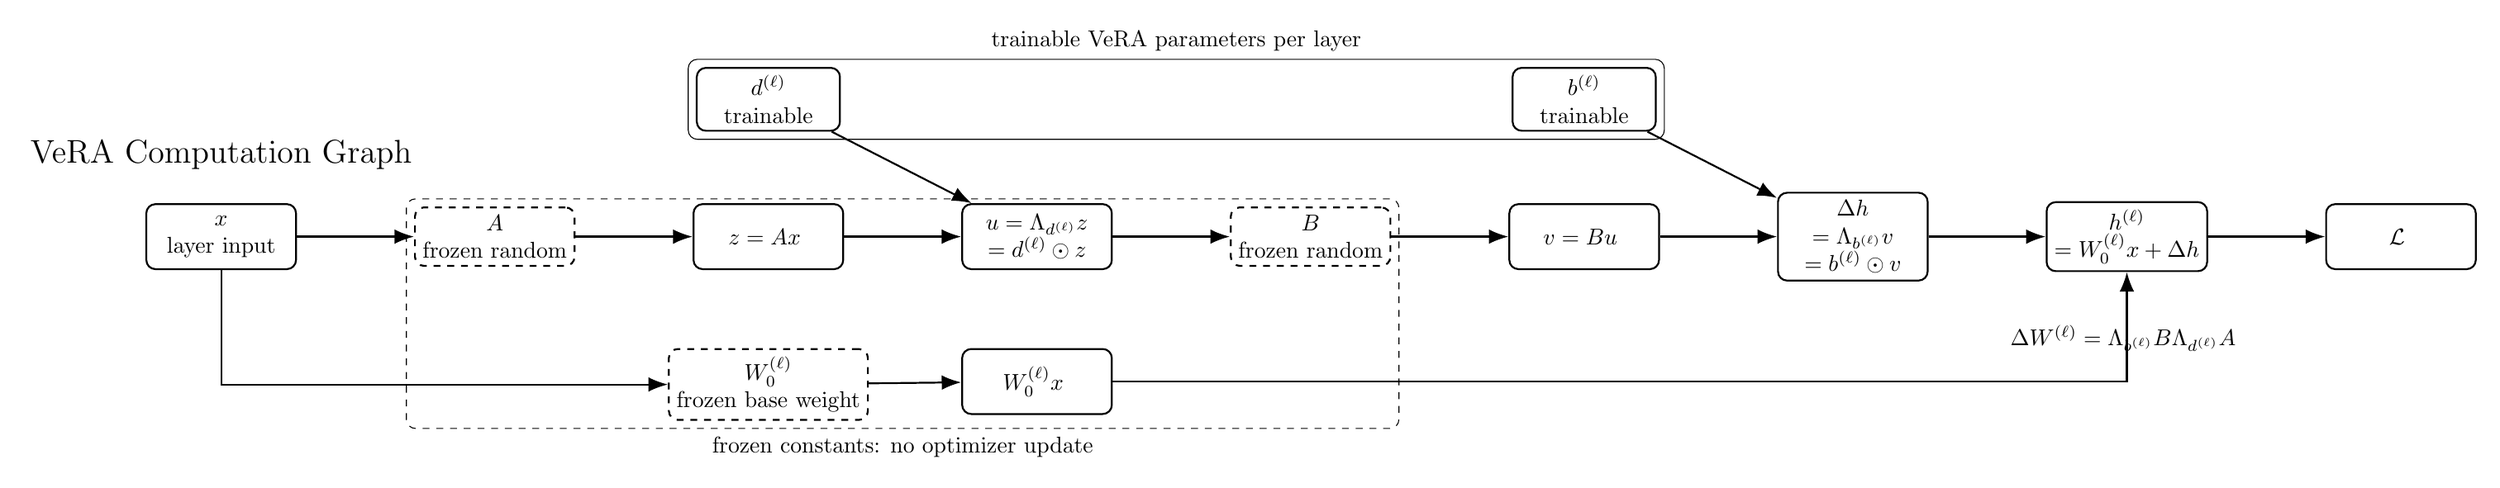
\begin{tikzpicture}[
		node distance=1.5cm and 1.8cm,
		box/.style={
			rectangle,
			rounded corners,
			draw,
			thick,
			align=center,
			minimum width=2.3cm,
			minimum height=1.0cm
		},
		frozen/.style={
			rectangle,
			rounded corners,
			draw,
			thick,
			dashed,
			align=center,
			minimum width=2.2cm,
			minimum height=0.9cm
		},
		trainable/.style={
			rectangle,
			rounded corners,
			draw,
			thick,
			align=center,
			minimum width=2.2cm,
			minimum height=0.9cm
		},
		arrow/.style={
			-{Latex[length=3mm]},
			thick
		},
		dashedarrow/.style={
			-{Latex[length=3mm]},
			thick,
			dashed
		}
		]
		
		\node[box] (x) {$x$\\layer input};
		
		\node[frozen, right=of x] (A) {
			$A$\\
			frozen random
		};
		
		\node[box, right=of A] (Ax) {
			$z=Ax$
		};
		
		\node[trainable, above=1.1cm of Ax] (d) {
			$d^{(\ell)}$\\
			trainable
		};
		
		\node[box, right=of Ax] (Dz) {
			$u=\Lambda_{d^{(\ell)}}z$\\
			$=d^{(\ell)}\odot z$
		};
		
		\node[frozen, right=of Dz] (B) {
			$B$\\
			frozen random
		};
		
		\node[box, right=of B] (Bu) {
			$v=Bu$
		};
		
		\node[trainable, above=1.1cm of Bu] (b) {
			$b^{(\ell)}$\\
			trainable
		};
		
		\node[box, right=of Bu] (Dbu) {
			$\Delta h$\\
			$=\Lambda_{b^{(\ell)}}v$\\
			$=b^{(\ell)}\odot v$
		};
		
		\node[frozen, below=1.2cm of Ax] (W0) {
			$W_0^{(\ell)}$\\
			frozen base weight
		};
		
		\node[box, below=1.2cm of Dz] (base) {
			$W_0^{(\ell)}x$
		};
		
		\node[box, right=1.8cm of Dbu] (h) {
			$h^{(\ell)}$\\
			$=W_0^{(\ell)}x+\Delta h$
		};
		
		\node[box, right=of h] (loss) {
			$\mathcal{L}$
		};
		
		\draw[arrow] (x) -- (A);
		\draw[arrow] (A) -- (Ax);
		\draw[arrow] (Ax) -- (Dz);
		\draw[arrow] (d) -- (Dz);
		\draw[arrow] (Dz) -- (B);
		\draw[arrow] (B) -- (Bu);
		\draw[arrow] (Bu) -- (Dbu);
		\draw[arrow] (b) -- (Dbu);
		\draw[arrow] (Dbu) -- (h);
		\draw[arrow] (h) -- (loss);
		
		\draw[arrow] (x) |- (W0);
		\draw[arrow] (W0) -- (base);
		\draw[arrow] (base) -| (h);
		
		\node[
		draw,
		dashed,
		rounded corners,
		fit=(A)(B)(W0),
		label=below:{frozen constants: no optimizer update}
		] {};
		
		\node[
		draw,
		rounded corners,
		fit=(d)(b),
		label=above:{trainable VeRA parameters per layer}
		] {};
		
		\node[above=0.4cm of x] {\Large VeRA Computation Graph};
		
		\node[below=0.7cm of h, align=center] {
			$\Delta W^{(\ell)}
			=
			\Lambda_{b^{(\ell)}}B\Lambda_{d^{(\ell)}}A$
		};
		
	\end{tikzpicture}
	
\end{document}